\papersubsection{Page management}
\label{sec:eval:pal:memory}

\begin{figure*}[t!]
\centering
\footnotesize
\resizebox{\textwidth}{!}{%
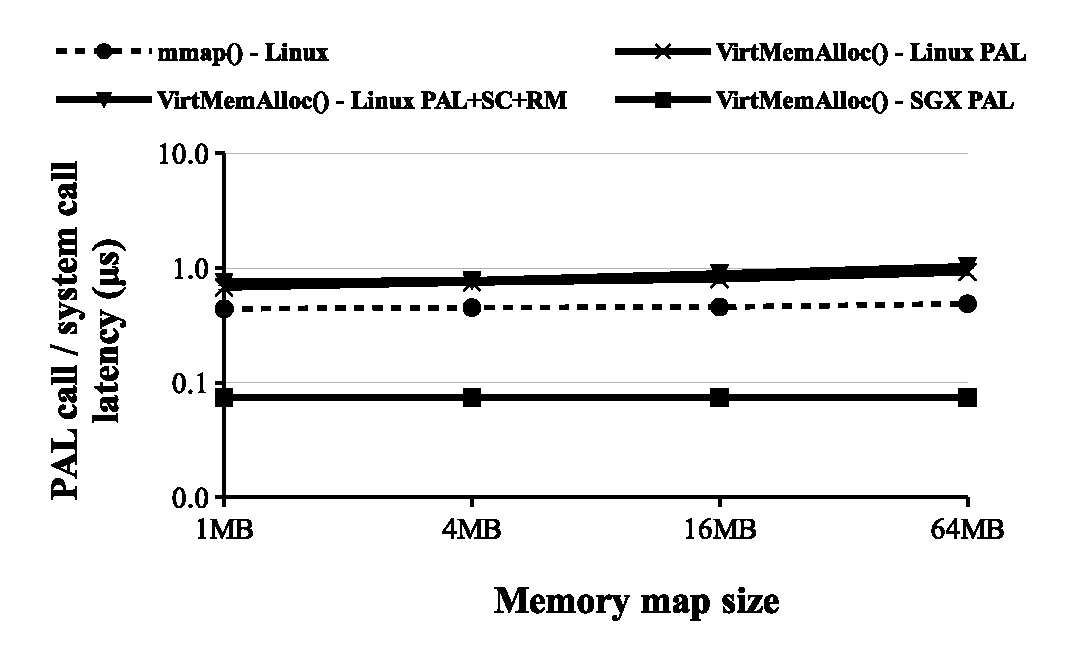
\includegraphics[height=10em]{mmap-latency}
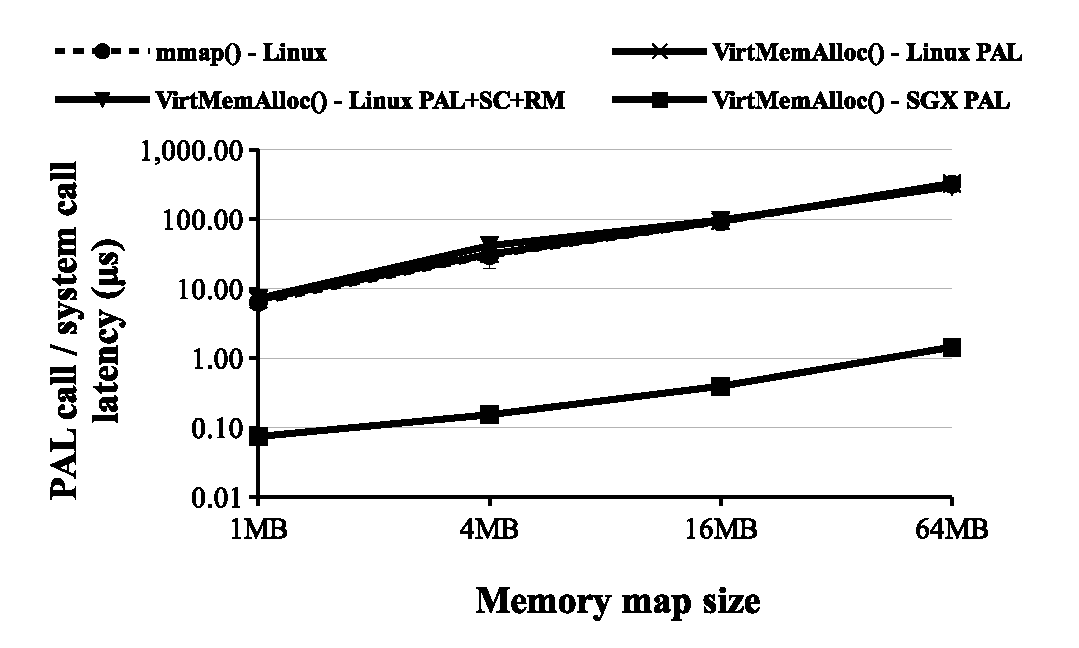
\includegraphics[height=10em]{mmap-access-latency}
}
\parbox{0.49\textwidth}{\centering\bf (a) allocation + deallocation}
\parbox{0.49\textwidth}{\centering\bf (b) allocation + memory access + deallocation}
\caption{Latency of (a) allocating and deallocating a range of virtual pages, and (b) the same operations with writing to each page after allocation. Lower is better.
The comparison is between (1) \syscall{mmap} and \syscall{munmap} on Linux; (2) \palcall{VirtMemAlloc} and \palcall{VirtMemFree} on the Linux PAL, with and without a \seccomp{} filter ({\bf +SC}) and reference monitor ({\bf +RM}); (3) the same \hostapis{} on the \sgx{} PAL, with and without zeroing the pages before use ({\bf +Zero}).}
\label{fig:eval:pal:mmap-latency}
\end{figure*}

%Unlike I/O streams, 
Single-process abstractions such as page management
tend to have less overheads
because no complex security check
is required.
%tend to have less impact on
%single-process \hostapis{}.
%Since updating page mappings only affects the process itself.
%any amount of anonymous pages within its resource limits.
In Figure~\ref{fig:eval:pal:mmap-latency},
the overheads of memory allocation and deallocation using \palcall{VirtMemAlloc} and \palcall{VirtMemFree}
over the native \syscall{mmap} and \syscall{munmap}
are almost negligible (less than 5\%),
even if the guest has accessed the allocated pages.
\graphene{} expects the same performance on any host OSes with dynamic page management.



%As the results on the Linux PAL represent the performance on a host with dynamic page management,
%Unlike a traditional OS like Linux,
The current \sgx{} PAL follows a static page management model,
due to the restriction of \sgx{} hardware.
For each enclave,
the \sgx{} PAL preallocate a heap space
at loading time,
and cannot update the enclave page layout
after the enclave starts. 
Although the untrusted OS still offer page-in and page-out
when an enclave requires more pages
than the EPC size (128MB in the current setup),
the \sgx{} PAL implements
internal page management to bypass the untrusted OS.
The latency
of allocating virtual pages, however,
is dominated by the cost of zeroing pages before returning to the guest.
Due to the memory access overheads in enclaves,
zeroing pages that are larger than the last-level cache size (4MB on a Intel i5-6500 CPU)
can be as expensive as 600-75,000\x{} to original \syscall{mmap} and \syscall{munmap} latency.
The \sgx{} version 2 hardware
can potentially improve the overheads by dynamically removing and adding pages to an enclave.
Without the memory zeroing cost,
page allocation and deallocation on the \sgx{} PAL
is only \roughly{}16\% to \syscall{mmap} and \syscall{munmap},
since the \sgx{} PAL
for simply updating the mappings
inside an enclave.
%the internal page mappings 
%without enclave exits.

%the \sgx{} PAL must manage its own pages since it does not trust the host OS.
%Therefore, the \sgx{} PAL maintains
%an internal VMA (virtual memory area) list,
%which is easily updated
%at a much lower latency (\roughly{}16\% to \syscall{mmap} and \syscall{munmap}).
 

%This section evaluates the performance of virtual page allocation and deallocation
%using \thehostabi{}.
%The latency of creating or destroying a virtual memory area
%may differ among PAL implementations
%due to different memory management models.
%The Linux PAL, for instance, has a memory management model
%similar to Linux,
%backed by demand paging.
%The \sgx{} PAL, on the other hand, has to preallocate all pages at loading time.
%Although the \sgx{} driver still swaps enclave pages,
%the latency of page-in and page-out can be up to 40,000 cycles~\cite{orenbach17eleos},
%%than normal page-in and page-out latency,
%and the current \sgx{} hardware does not allow dynamically adding pages
%to an enclave.
%As a result, the \sgx{} PAL includes an in-enclave memory allocator
%which manages unused enclave pages
%and assigns the pages to memory allocation requests.
%To evaluate
%the differences of memory management models,
%the experiments
%include two scenarios:
%(1) simply allocating and deallocating virtual pages;
%(2) allocating virtual pages,
%accessing the beginning of every pages,
%and then deallocating the pages.
%For each scenario,
%the benchmark tests with different memory mapping sizes.








%Figure~\ref{fig:eval:pal:mmap-latency} (a)
%shows the latency of
%simple allocation and deallocation.
%Linux and the Linux PAL
%show similar latency for allocating and deallocating any numbers
%of virtual pages,
%as the cost of updating the page table
%in the host kernel.
%For the Linux PAL, the latency
%of \palcall{VirtMemAlloc} and  \palcall{VirtMemFree} is 50--80\% higher
%than \syscall{mmap} and \syscall{munmap} on Linux
%(the overheads of \seccomp{} filter and reference monitor is negligible).
%For the \sgx{} PAL,
%the latency of allocation and deallocation
%is much lower,
%at \roughly{}10\% of the latency of \syscall{mmap} and \syscall{munmap}.
%%since the enclave simply
%%updates the bookkeeping inside the page allocator
%%and never exits the enclave.
%However,
%since \sgx{} doesn't guarantee the initial state of unmeasured enclave pages,
%the \sgx{} PAL needs to zero all pages
%before passing to the guest.
%Accessing the pages after allocation
%may cause cache misses and enclave page swapping,
%when the allocation size
%is larger than the size of last-level cache.
%The result shows that,
%if the \sgx{} PAL zeros pages after allocation,
%the latency of allocation and deallocation can increase by up to several orders of magnitude.
%%be order-of-magnitude higher than \syscall{mmap} and \syscall{munmap}.



%If the latency includes accessing every pages in between allocation and deallocation,
%as shown in Figure~\ref{fig:eval:pal:mmap-latency} (b),
%the overall latency (including allocating, access, and deallocating pages) would
%naturally be proportional to the allocation size.
%The benchmark results show almost no difference
%between the latency on the Linux PAL and in a native Linux process.
%Because the benchmark only access the first words
%of every pages,
%the latency on the \sgx{} PAL without page zeroing
%is still lower than the Linux PAL.
%If the \sgx{} PAL zeros the pages after allocation,
%accessing the first words
%of every pages causes no additional overheads
%on the overall latency.




